\chapter{COMET Phase-I Sensitivity and Background Estimates}
\label{ch:phase-I_study}

With the framework to simulate backgrounds from atmospheric muons in place, we
can now combine the results into a complete sensitivity and background
simulation study for COMET Phase\nobreakdash-I. In this chapter, we discuss our
simulation samples consisting of signal, decay in orbit (DIO), and atmospheric
events, and present our resulting expectations of the performance of
Phase\nobreakdash-I. All data samples simulated for this study were produced
on the CC-IN2P3 cluster.

\section{Data samples}
Three simulation samples are produced for this study: a $\mu$--$e$ conversion
sample, a DIO sample and an atmospheric muon sample. All three are simulated in
the geometrical world shown in Figure~\ref{fig:bmc_geometry}. This geometry
differs from the older TDR design~\cite{the_comet_collaboration_comet_2020} by
the number of counters in the CTH. Here, each layer of the CTH has 64 counters
instead of the original 48, which mainly affects the detector's geometrical
acceptance. In addition, we use the first-stage layout of the CTH, where both
layers are composed entirely of plastic scintillation counters. In contrast, the
final stage will have Cherenkov counters in the outer layer. As we shall see,
this has a considerable impact on the detector's ability to discriminate
atmospheric muons from conversion electrons.

\subsection{\texorpdfstring{$\mu$--$e$}{Muon-to-electron} conversion} 

\subsubsection{Sample}

The signal sample is the most straightforward to produce. We initially generate
primary electrons with energy $E=\SI{104.97}{\MeV}$ uniformly inside the
stopping target disks. Their direction is isotropically distributed, as would be
the case in the conversion process. A uniform position distribution in each disk
is not realistic, because the actual distribution depends on where in the
stopping target the muons in the beam come at rest. To account for this, the
events are weighted according to the stopping positions of muons recorded in the
MC5 simulation. The weighting factor is determined from the relative probability
for a muon to stop at the sampled position, which is estimated by histogramming
the stopping positions in each disk.
Figure~\ref{fig:stopping_position_reweighting} shows the initially-sampled
uniform position distribution, the muon stopping position distribution from MC5,
and the result of event weighting. In total, $N_\mathrm{signal} =
2\times 10^6$ events are simulated to compose the signal sample.

% After applying geom cut of CTH trigger, how many remain?

\begin{figure}
    \centering
    \begin{subfigure}[t]{0.329\textwidth}
        \centering
        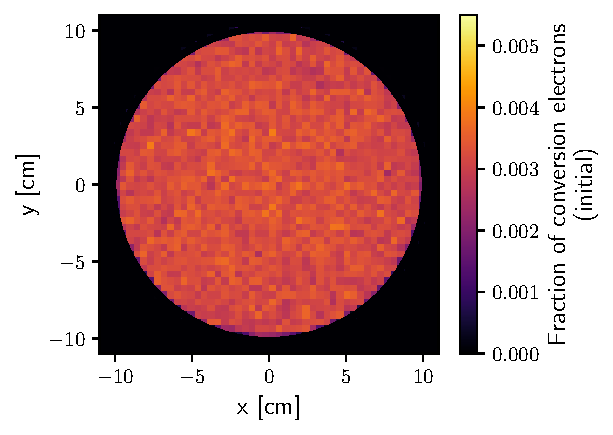
\includegraphics[width=\textwidth]{chapter6/initial_conversion_position_distribution.pdf}
        \caption{Pre-weighting.}
    \end{subfigure}
    \hfill
    \begin{subfigure}[t]{0.329\textwidth}
        \centering
        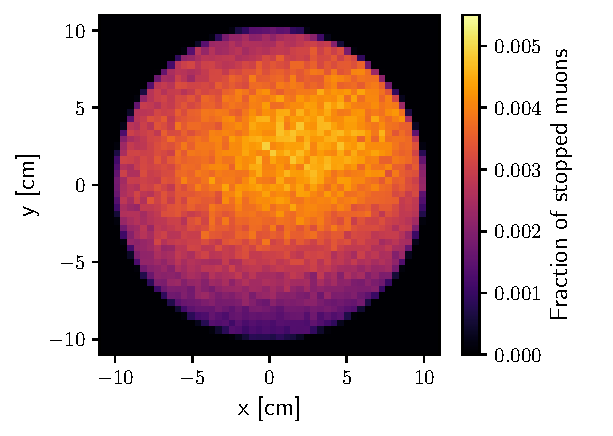
\includegraphics[width=\textwidth]{chapter6/stopped_muon_distribution.pdf}
        \caption{Bound muon position distribution from MC5 used as weight.}
    \end{subfigure}
    \hfill
    \begin{subfigure}[t]{0.329\textwidth}
        \centering
        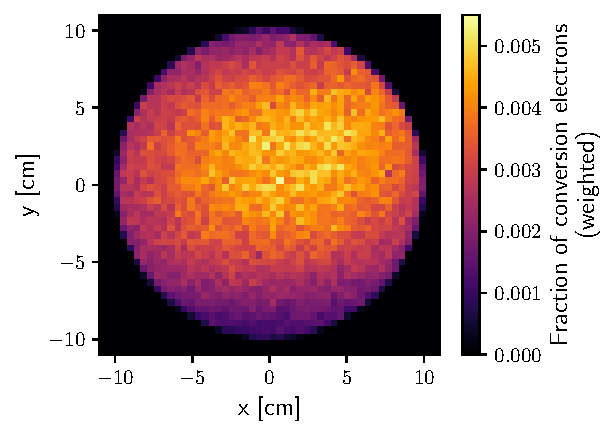
\includegraphics[width=\textwidth]{chapter6/weighted_conversion_position_distribution.pdf}
        \caption{Post-weighting.}
    \end{subfigure}
    \caption{ Initial position distribution of signal electrons before and after
        weighting them by the likelihood of a muon being bound in each bin. }
    \label{fig:stopping_position_reweighting}
\end{figure}


\subsubsection{Selection}
Signal events are selected based on detector acceptance criteria. We first
require fourfold coincidence in the CTH. Figure~\ref{fig:cydet_signal_event}
shows an example of a conversion event which passes this trigger criterion. The
fraction of events remaining defines the geometrical acceptance 
\begin{equation}
A_\mathrm{geom} \equiv  \frac{N_\text{4-fold}}{N_\mathrm{signal}}.
\end{equation}
In this simulation, the estimated geometrical acceptance is $A_\mathrm{geom} =
\SI{21}{\percent}$. In comparison, the TDR cites $A_\mathrm{geom} =
\SI{26}{\percent}$ with the previous design of the CTH.


% Reconstruction
We do not fully simulate the reconstruction of signal electron trajectories in
the CDC. In order to approximate the effect of reconstruction uncertainties, a
smearing is applied to the true momentum of each track. The reconstructed
momentum is estimated as $p_r = p_t + x$, where $p_t$ is the true momentum of
the electron as it enters the CDC, $x \sim \mathcal{N}(0, \sigma)$, and $\sigma
= \SI{200}{\keV/\clight}$ is the expected momentum resolution of the CDC. Since
tracks are not properly reconstructed, we do not apply any track quality cuts to
select events but instead weight the signal sample by the associated acceptance
factor from Table~\ref{tab:acceptance} to account for the rejection of some
events.

In this simulation sample, the initial time for each event does not correspond
to the realistic time distribution of the $\mu$--$e$ conversion process. Hence,
events are not selected based on whether they reach the detector within the
trigger time window, but we weight the sample by the trigger time window
efficiency factor instead. Similarly, the sample is weighted by the trigger and
data acquisition efficiency factors to account for the loss of acceptance from
hardware effects. Table~\ref{tab:acceptance} lists the values of these
efficiency factors.


\subsection{Muon decay in orbit}
\subsubsection{Sample}
The DIO sample is similar to the signal sample in that the initial position
of signal and DIO electrons is identically distributed. Hence, we also sample
uniformly in the stopping target disks and then weight the events according to
the MC5 stopping position distribution. Similarly, the direction of DIO
electrons is sampled isotropically. The energy distribution is thus the only
difference between the two samples. 

\begin{figure}
    \centering
    \begin{subfigure}[t]{0.4\textwidth}
    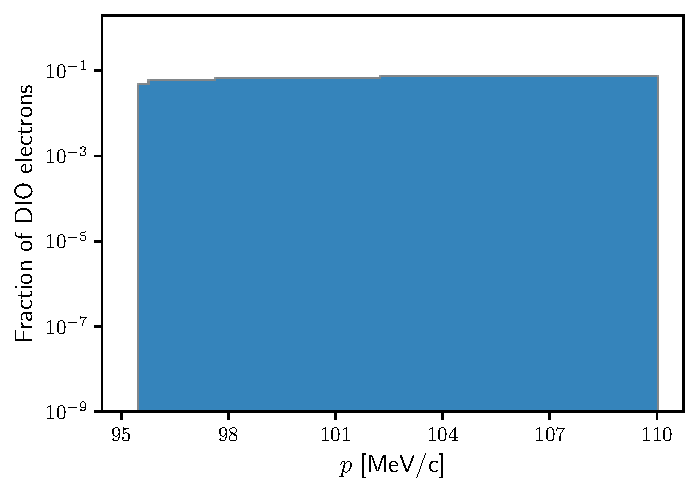
\includegraphics[width=\textwidth]{chapter6/dio_momentum_distribution_initial.pdf}
    \caption{Initial sampling.}
\end{subfigure}
    \hspace{2cm}
    \begin{subfigure}[t]{0.4\textwidth}
        \centering
        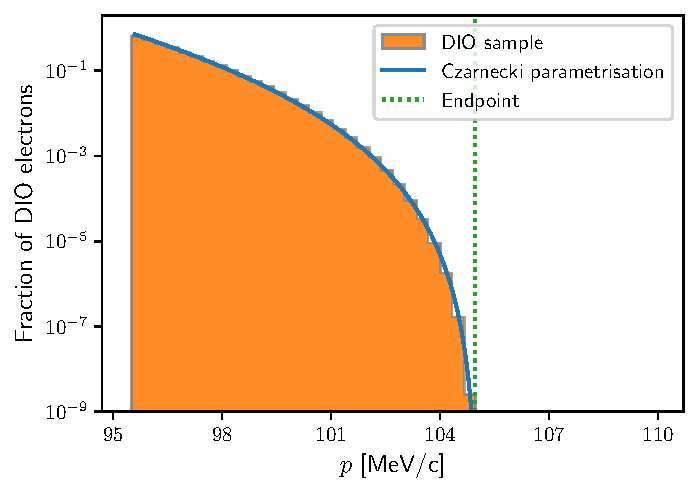
\includegraphics[width=\textwidth]{chapter6/dio_momentum_distribution_czarnecki_weighted.pdf}
        \caption{Weighted with the Czarnecki et al. parametrisation~\cite{czarnecki}.}
    \end{subfigure}
    \caption{Momentum spectrum of electrons in the DIO sample.}
    \label{fig:czarnecki_spectrum}
\end{figure}

The theoretical energy spectrum of DIO electrons produced in aluminium muonic
atoms was investigated by Czarnecki et al.~\cite{czarnecki}. Here, we use their
proposed parametrisation of the energy spectrum around the DIO energy endpoint:
\begin{equation}\label{eq:czarnecki_param}
P(E_e) = a_5 \delta^5 + a_6 \delta^6 + a_7 \delta^7 + a_8 \delta^8,
\end{equation}
where $\delta \equiv E_\mu  - E_e - \frac{E_e^2}{2 m_\mathrm{Al}}$, $E_\mu =
\SI{105.194}{\MeV}$, $m_\mathrm{Al} = \SI{25133}{\MeV}$, with the values of the
four $a$ coefficients provided by the authors. This approximation is valid in
the region $E_e > \SI{85}{\MeV}$, which is sufficient to cover our whole DIO
sample. We use this spectrum parametrisation to weight DIO events based on their
energy. Similarly to the position weighting procedure, DIO events are first
generated with a uniform energy distribution in the range $E \in [95,
110]~\si{\MeV/\clight}$, and then weighted according to the probability for a
DIO electron to have the sampled energy. Figure~\ref{fig:czarnecki_spectrum}
shows the momentum spectrum of DIO electrons before and after weighting.

The DIO sample is composed of $N_\mathrm{DIO} = 10^7$ events in total.
Figure~\ref{fig:muon_dio_in_cydet} shows an example of a potential background
event from DIO where an electron with an energy close to the conversion energy
flies into the CyDet system and activates the trigger.

\begin{figure}
    \centering
    %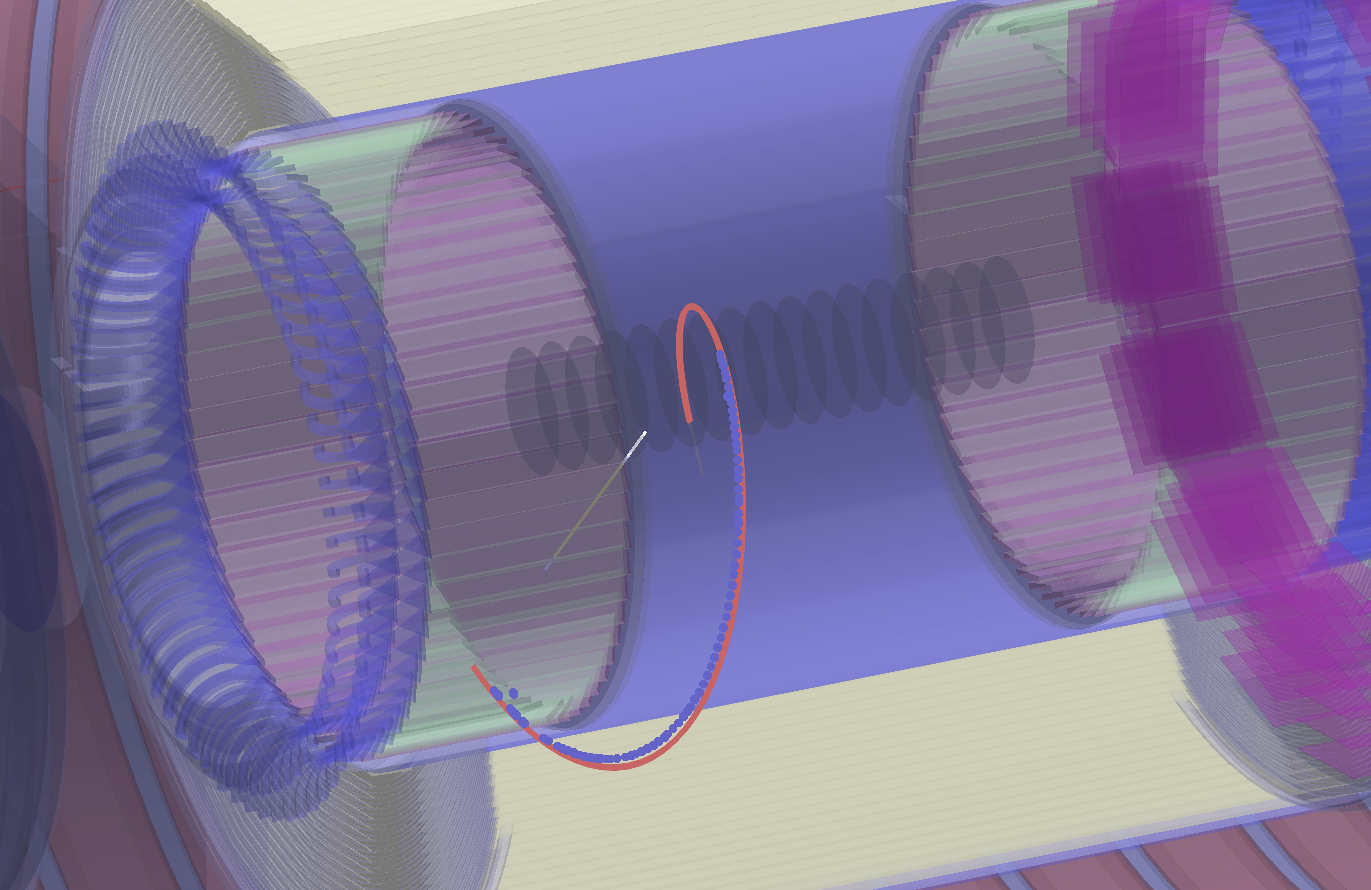
\includegraphics[width=0.6\textwidth]{chapter6/dio_event_in_cydet.png}
    % Event 469 in first DIO_95 root file
    \begin{subfigure}{0.522\textwidth}
        \centering
        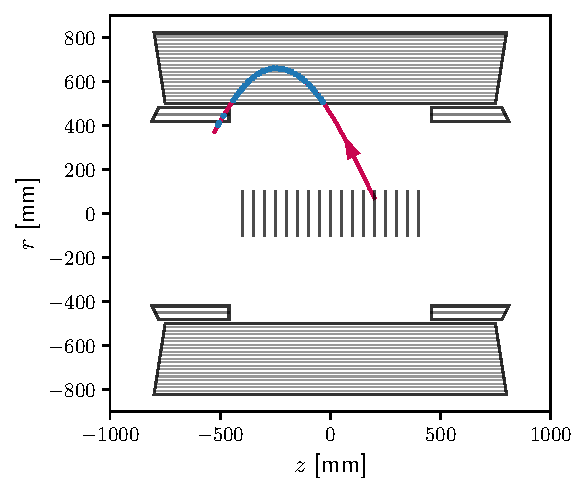
\includegraphics[width=\textwidth]{chapter6/dio_track_zy.pdf}
        \caption{$z$--$r$ projection, where $r = \sqrt{x^2+y^2}$.}
    \end{subfigure}
    \hfill
    \begin{subfigure}{0.467\textwidth}
        \centering
        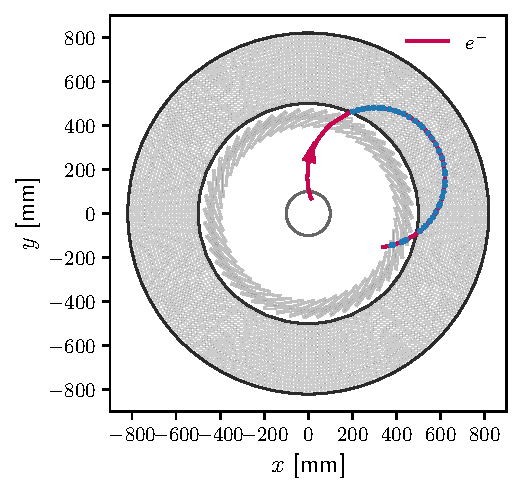
\includegraphics[width=\textwidth]{chapter6/dio_track_xy.pdf}
        \caption{$x$--$y$ projection.}
    \end{subfigure}
    \caption{ Potential DIO-induced background with momentum
        $p=\SI{103.7}{\MeV/\clight}$.}
    \label{fig:muon_dio_in_cydet}
\end{figure}

\subsubsection{Selection}
The selection of DIO events is identical to the selection of conversion events.
We require a fourfold coincidence in the CTH, and then apply a Gaussian smear to
the true momentum of the electron to approximate track reconstruction. The same
efficiency and acceptance factors as for signal events are applied to weight the
sample and determine the absolute background contribution from the DIO process.


\subsection{Atmospheric muons}

\subsubsection{Sample}

Atmospheric muon events are simulated as discussed in
Section~\ref{sec:cosmic_event_sampling}. Two samples are produced, one around the
entire surface of the CRV and one more densely concentrated on its upstream and
downstream openings. Because of how rarely a sampled atmospheric event produces
signal-like features, the atmospheric dataset is the largest of the three, with
$1 \times 10^9$ events generated on the envelope and $1.4 \times 10^9$ on the
openings.


\begin{figure}
    \centering
    %\includegraphics[width=0.6\textwidth]{chapter6/sneaking_mu-_event_0.png}
    \begin{subfigure}{0.56\textwidth}
        \centering
        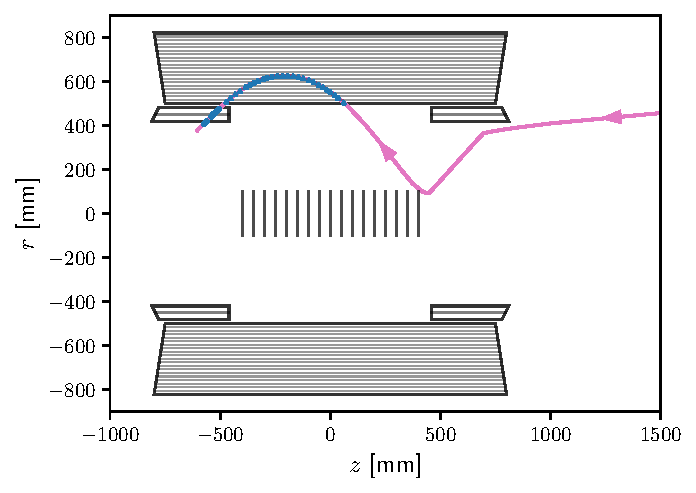
\includegraphics[width=\textwidth]{chapter6/mu-_track_zy.pdf}
        \caption{$z$--$r$ projection, where $r = \sqrt{x^2+y^2}$.}
    \end{subfigure}
    \hfill
    \begin{subfigure}{0.43\textwidth}
        \centering
        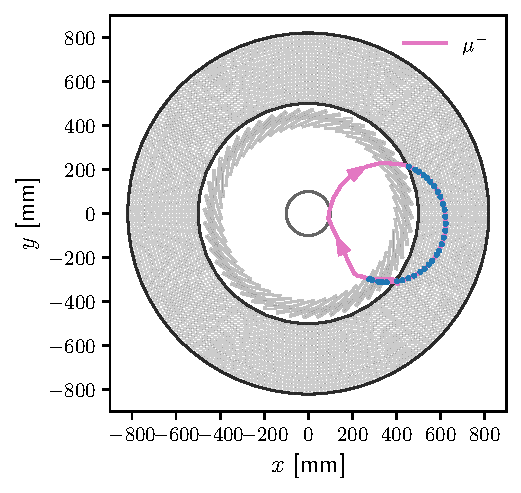
\includegraphics[width=\textwidth]{chapter6/mu-_track_xy.pdf}
        \caption{$x$--$y$ projection.}
    \end{subfigure}
    % Event 22855 in run 7833 
    % (select_sneaking_DSoffset_7000-7999_checkveto+cdc.root.json)
    % Fitted momentum: 105.5 MeV/c
    \caption[Sneaking atmospheric $\mu^-$ background]{ Sneaking atmospheric
        $\mu^-$ background with a reconstructed momentum
        $p=\SI{103.5}{\MeV/\clight}$. The muon enters through the downstream
        opening of the CRV and scatters in the aluminium CTH support structure.
        Then, it produces a track in the CDC and a fourfold coincidence in the
        CTH. Importantly, the trajectory crosses the muon stopping target,
        making it more difficult to distinguish from the conversion signal. }
    \label{fig:cosmic_muon_bg_in_cydet}
\end{figure}

\subsubsection{Selection}
As for signal and DIO events, atmospheric events must at least pass the fourfold
coincidence criterion. Unlike signal and DIO events, hit information from the
CDC is also used to select track candidates. Two criteria apply: the particle
must reach at least the 5th innermost layer of the CDC, but it should not hit
the outermost layer. Hence, we select tracks with sufficient transverse
momentum to be reconstructed, but reject tracks that either have too large a
momentum to be a signal event, or appear to enter the CDC from the outside. 

In addition, the hit positions are used to reconstruct the track using a helix
fit. The fitted trajectory should intersect the muon stopping target to pass the
selection. Figure~\ref{fig:cosmic_muon_bg_in_cydet} shows an example of such an
atmospheric event. The helix fit estimates the momentum of the particle, which
is used in the analysis stage. Hence, for this sample, we do not apply a
Gaussian smear to the true momentum but use the estimated momentum from the fit
instead.

\subsubsection{Rate estimation}
As discussed in Section~\ref{sec:bmc_conversion_bg_rate}, the rate for each selected
event is estimated by backward MC simulation. The backward propagation and flux
sampling is repeated 5000 times for every event, which yields an average flux
and a statistical error shown in the results.


\subsection{Sample weighting}\label{sec:sample_weighting}
\sepfootnotecontent{fn:conv_br_norm}{The nuclear muon capture branching ratio appears in this
expression because the branching ratio of $\mu$--$e$ conversion is
conventionally normalised to $\mathcal{B}_\mathrm{capture}$.}

Because they originate from different processes, the three MC samples must be
individually weighted in order to determine the absolute contribution from each.
The conversion and DIO processes both originate from the muons bound in the
stopping target, hence we can express the total number of expected conversion
and DIO electrons in terms of the total number of stopped muons $N_\mu$.
The number of signal electrons, as a function of the conversion branching
ratio $\mathcal{B}_\mathrm{conversion}$, is:
\begin{equation}\label{eq:weight_signal}
N_\mathrm{conversion} = 
N_\mu \, \mathcal{B}_\mathrm{conversion} \, 
\mathcal{B}_\mathrm{capture} \, f_\mathrm{coherent},
\end{equation}
where $\mathcal{B}_\mathrm{capture} = 0.61$ is the branching ratio of nuclear
muon capture\sepfootnote{fn:conv_br_norm} and $f_\mathrm{coherent}=0.9$ is the
fraction of conversions that are coherent.

Similarly, the total number of DIO electrons can be expressed as:
\begin{equation}
N_\mathrm{DIO} = N_\mu \, \mathcal{B}_\mathrm{DIO},
\end{equation}
where $\mathcal{B}_\mathrm{DIO} = 1 - \mathcal{B}_\mathrm{capture} = 0.39$ is
the branching ratio of DIO. Our simulation sample, however, only covers the part
of the DIO spectrum where $E_e > \SI{95}{\MeV}$, so we cannot simply use
$N_\mathrm{DIO}$ as the sample weight. The proper weight is given by 
\begin{align}\label{eq:weight_dio}
N_\mathrm{DIO}^{p>\SI{95}{\MeV}} &= N_\mathrm{DIO} \, P(E_e > \SI{95}{\MeV}) \\\nonumber
&= N_\mathrm{DIO}\,\int_{\SI{95}{\MeV}}^{E_\mathrm{endpoint}} P(E_e)\,dE_e,
\end{align}
where $E_\mathrm{endpoint} = \SI{104.973}{\MeV}$ is the energy above which no
DIO electron can be produced. The integral term in this equation is estimated by
numerically integrating the Czarnecki parametrisation of
Equation~\ref{eq:czarnecki_param}.
%  to obtain $N_\mathrm{DIO}^{p>\SI{95}{\MeV}} = 0.67$ assuming $N_\mu = 1.5e16$.

In the case of atmospheric muons, the backward MC procedure yields an absolute
rate $R$ for each event. This rate can simply be integrated over the total
data acquisition time of the experiment $T_\mathrm{DAQ}$ to obtain the expected
event count:
\begin{equation}\label{eq:weight_atmospheric}
N_\mathrm{atmospheric} = \int_0^{T_\mathrm{DAQ}} R\,dt = R \times T_\mathrm{DAQ}.
\end{equation}

In the TDR, COMET Phase\nobreakdash-I was estimated to reach its sensitivity goal for
$T_\mathrm{DAQ} = 146$~days. In this study, we keep this value fixed to be able
to compare our sensitivity and background estimates with the original study.
%This run time
%corresponds to $N_\mu = 1.5 \times 10^{16}$. In the subsequent analysis, we
%substitute these two values into
%Equations~\ref{eq:weight_signal},~\ref{eq:weight_dio}
%and~\ref{eq:weight_atmospheric} to weight each sample.



\subsubsection{Trigger time window efficiencies}
In order to take into account the trigger timing window, we assume that
atmospheric muons irradiate the detector with a uniform time distribution.
Hence, the time window efficiency factor is the average fraction of time when
the trigger is active:
\begin{equation}
\epsilon_\text{time window}^\mathrm{atmospheric} =
\frac{8}{9}\,\frac{1170 - 700}{1170} = \SI{36}{\percent}
\end{equation}
assuming the trigger window is between 700 and \SI{1170}{\ns}, and where the
factor $\frac{8}{9}$ arises from the bunch structure of the J-PARC main ring. In
contrast, the efficiency factor for conversion and DIO electrons
$\epsilon_\text{time window}^\text{conversion|DIO} = \SI{30}{\percent}$ is
smaller because the time distribution of bound muons is not uniform but peaks
around \SI{300}{\ns}, before the trigger becomes active (see
Figure~\ref{fig:timing_distributions}).



\section{Single event sensitivity}
As discussed in Section~\ref{sec:SES}, the single event sensitivity (SES) is
defined as the value of the $\mu$--$e$ conversion branching ratio required for
the experiment to observe one signal event. It can be expressed in terms of the
experimental acceptance $A_{\mu-e}$ and the total number of muons stopped in the
stopping target $N_\mu$:
\begin{equation}
\mathrm{SES} = 
\frac{1}{N_\mu\,A_{\mu-e}\,\mathcal{B}_\mathrm{capture}\,f_\mathrm{coherent}},
\end{equation}
where $\mathcal{B}_\mathrm{capture} = 0.61$ and $f_\mathrm{coherent} = 0.9$.

In this simulation study, we found the geometrical acceptance $A_\mathrm{geom}$
of the CyDet with the new CTH layout to be reduced from \SI{26}{\percent} to
\SI{21}{\percent}. Hence, the net signal acceptance $A_{\mu-e}$ decreases from
\SI{4.1}{\percent} to \SI{3.3}{\percent}. On the other hand, the yield of
stopped muons per proton collision was estimated from the MC5 dataset to be
$R_{\mu / p} = 4.86 \times 10^{-4}$, which is slightly higher than the TDR
value. Overall, although the total number of bound muons is increased for the
same run time, it is outweighed by the decrease in acceptance. Keeping
$T_\mathrm{DAQ}$ fixed at 146 days, we obtain $N_\mu = 1.53 \times 10^{16}$,
hence our estimation of the COMET Phase\nobreakdash-I sensitivity is
\begin{equation}
\mathrm{SES} = 3.6 \times 10^{-15}.
\end{equation}

\subsection*{Uncertainties}
The above estimate comes with an uncertainty which depends most heavily on our
uncertain knowledge of the proton beam and the exact yield of backward-moving
pions after the collision, both of which impact $N_\mu$. Other factors are involved,
such as the accuracy of our acceptance estimate $A_{\mu-e}$, and the theoretical
uncertainty on $\mathcal{B}_\mathrm{capture}$ and $f_\mathrm{coherent}$.

In order to determine the uncertainty on $N_\mu$, one would have to carefully
determine how much it fluctuates with respect to changes in the proton beam
profile which we use to generate events. The change in $N_\mu$ with respect to
the backward-emitted pion yield would also have to be investigated. One could
then propagate uncertainty in our knowledge of the beam and its collision to the
total number of muons that will come at rest in the stopping target.

Concerning the acceptance estimate $A_{\mu-e}$, many of its factors were derived
from prior simulation studies and the final value adjusted to account for known
differences. In the future, we hope that a complete estimation based on
realistic detector, electronics and reconstruction simulations can be performed.
An uncertainty could then be derived for $A_{\mu-e}$ which would include our
confidence in the calibration, reconstruction and event selection procedures.



\section{Signal and background event counts}

After applying the efficiency factors and weighting each sample by the total
number of expected events as per Section~\ref{sec:sample_weighting}, we are able
to determine the absolute contribution from each source over a given data
acquisition period.

\subsection{Momentum spectrum}

\begin{figure}
    \centering
        
    \begin{subfigure}[t]{0.49\textwidth}
        \centering
        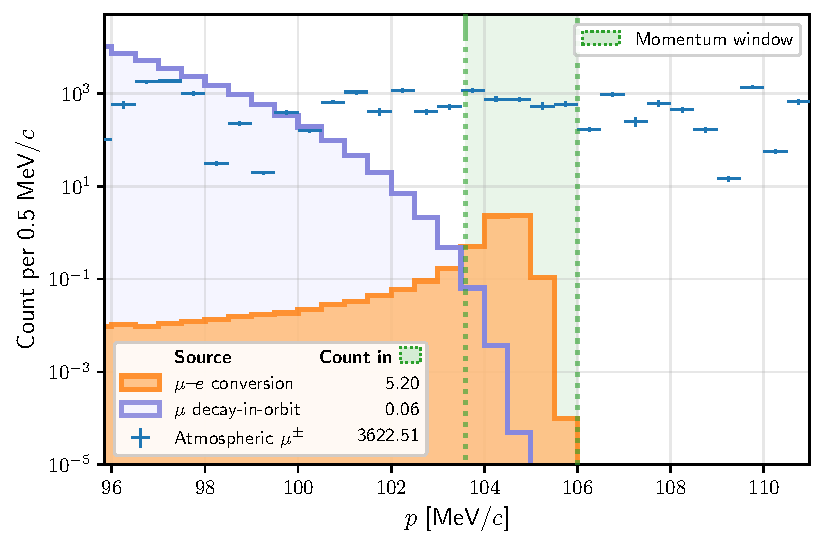
\includegraphics[width=\textwidth]{
            chapter6/thesis_conversion_search_momentum_distribution_nocuts_v5.pdf}
            \caption{ Without $\mu^\pm$ identification by the CRV, timing window
            cuts or track quality cuts. }
        \label{fig:log_spectrum_nocuts}
    \end{subfigure}
    \hfill
    \begin{subfigure}[t]{0.49\textwidth}
        \centering
        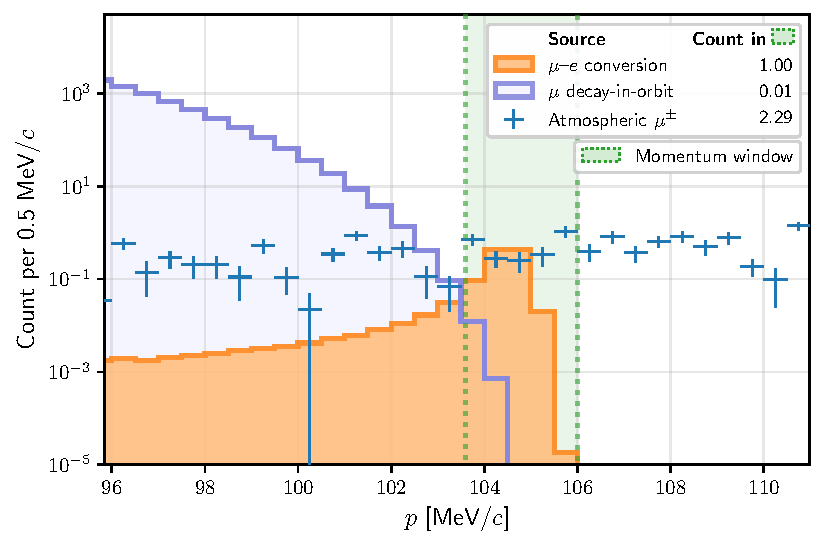
\includegraphics[width=\textwidth]{chapter6/thesis_conversion_search_momentum_distribution_withcuts_except_directionID.pdf}
        \caption{ With \SI{99.99}{\percent} $\mu^\pm$ rejection by the CRV,
        timing and track quality cuts. }
        \label{fig:log_spectrum_cuts_except_directionID}
    \end{subfigure}
    \caption[Momentum spectrum of conversion, DIO and atmospheric events around
    the conversion energy]{ Momentum spectrum of conversion, DIO and atmospheric
    events around the conversion energy, integrated over the Phase-I run time
    $T_\mathrm{DAQ} = 146$~days, assuming $\mathcal{B}_\mathrm{conversion} =
    3.61\times 10^{-15}$. Error bars on the atmospheric event bins show the
    statistical uncertainty from the backward MC flux estimation.
    % For atmospheric events, we compare the absence and presence of
    % the CRV in rejecting backgrounds. We also show the effect of the time
    % trigger window and track quality cuts on the signal and DIO contributions. 
    }
    \label{fig:log_spectra}
\end{figure}


The absolute event counts from conversion, DIO and atmospheric muon events are
plotted as a function of the reconstructed track momentum in
Figure~\ref{fig:log_spectra}. Note again that for conversion and DIO, $p$ is the
smeared momentum of the electron as it enters the CDC, whereas we use the
momentum reconstructed via a helix fit for atmospheric muon events.


In order to determine the effect of the CRV on the atmospheric background, as in
Figure~\ref{fig:log_spectrum_cuts_except_directionID}, we apply a weight to each
event based on whether it passed through the active material of the CRV. For
events that produce hits in the CRV, the weight is the assumed inefficiency of
the CRV: $1 - (\SI{99.99}{\percent}) = 10^{-4}$. Events that sneak into the
detector are given a weight of 1 since the CRV cannot veto them. Similarly, to
simulate the absence of the CRV, as in Figure~\ref{fig:log_spectrum_nocuts}, all
atmospheric muon events have a weight of 1, corresponding to a
\SI{0}{\percent}-efficient CRV.



\sepfootnotecontent{fn:bg_study_rmc}{ We chose not to show the radiative muon
    capture spectrum in our plots because the contribution from RMC is smaller
    than that of DIO by a factor of 5~\cite{the_comet_collaboration_comet_2020}.
}



% However, by investigating where
% these background events come from, we will see that there are ways to identify
% some of them and reduce their contribution below the single-event threshold.

The momentum of the candidate track is one of the most important criteria in
distinguishing signal electrons from DIO or RMC\sepfootnote{fn:bg_study_rmc}
electrons, because the energy spectra of the latter two fall off sharply close
to the conversion energy. In Phase\nobreakdash-I, the momentum window within which an event
is counted is $p \in [103.6, 106.0]\,\si{\MeV/\clight}$. This cut eliminates the
majority of DIO and RMC backgrounds. However, atmospheric background events
appear to be uniformly distributed in this range, making the cut ineffective in
rejecting them. 

Figure~\ref{fig:log_spectrum_nocuts} shows that in the absence of the CRV,
atmospheric backgrounds overwhelm the detector and outnumber conversion events
by three orders of magnitude in the momentum window. In the presence of the CRV,
and assuming an efficiency of \SI{99.99}{\percent}
(Figure~\ref{fig:log_spectrum_cuts_except_directionID}), atmospheric backgrounds
are suppressed by a factor $10^3$. However, their integrated count still exceeds
one, making the $\mu$--$e$ conversion search impossible unless there is an
additional way to identify them.


% For the atmospheric sample, we also reduce the background rate of certain events
% based on the primary particle ($\mu^-$ or $\mu^+$) and whether they hit the CRV.
% The first stage of the CTH, containing only scintillation counters and no
% Cherenkov counters, is unable to differentiate muons from electrons. Hence,
% signal-like tracks induced by sneaking atmospheric $\mu^+$ are a major source of
% backgrounds in this situation. 






\subsection{Particle identification}
%\subsection{Atmospheric \texorpdfstring{$\mu^+$}{anti-muon} backgrounds and particle identification}


\begin{figure}
    \centering
    %\includegraphics[width=0.6\textwidth]{chapter6/sneaking_mu+_event_2.png}
    \begin{subfigure}{0.56\textwidth}
        \centering
        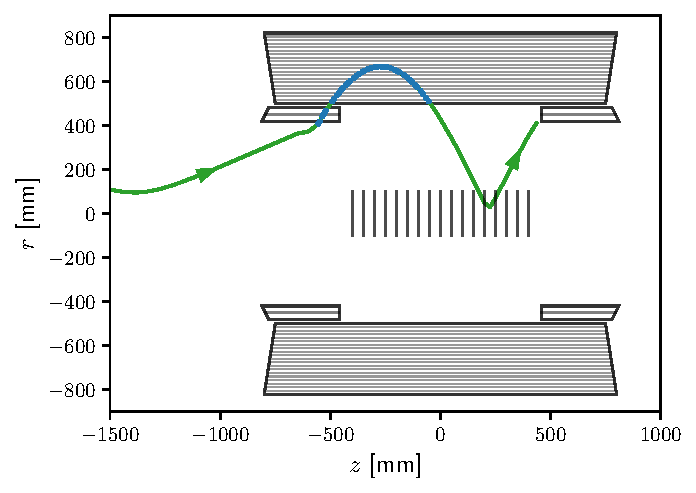
\includegraphics[width=\textwidth]{chapter6/mu+_track_zy.pdf}
        \caption{$z$--$r$ projection, where $r = \sqrt{x^2+y^2}$.}
    \end{subfigure}
    \hfill
    \begin{subfigure}{0.43\textwidth}
        \centering
        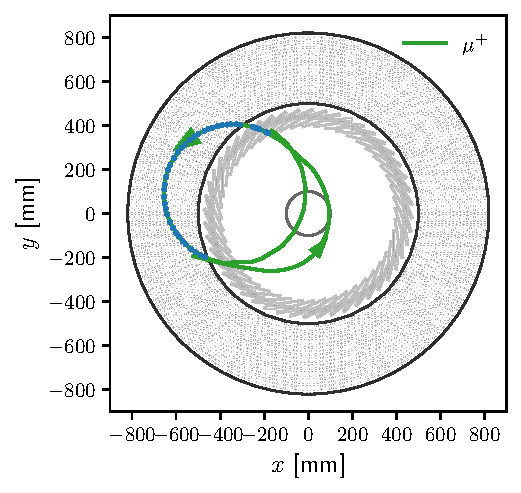
\includegraphics[width=\textwidth]{chapter6/mu+_track_xy.pdf}
        \caption{$x$--$y$ projection.}
    \end{subfigure}
    % Event 22855 in run 7833 
    % (select_sneaking_DSoffset_7000-7999_checkveto+cdc.root.json)
    % Fitted momentum: 90.3 MeV/c
    \caption[Sneaking atmospheric $\mu^+$ background event]{ Sneaking
        atmospheric $\mu^+$ background. It enters through the upstream opening
        of the CRV and scatters in the aluminium CTH support structure before
        inducing a fourfold coincidence in the CTH, producing a signal-like
        track in the CDC, and flying through the muon stopping target. The
        anti-muon thus appears as a time-reversed signal-like event. }
    \label{fig:cosmic_antimuon_bg_in_cydet}
\end{figure}

% TODO: read this over and remove ref to Moritsu
So far, we have assumed that the CyDet system has no way of discriminating
between electrons, muons, and anti-muons. However, this is not accurate. At
a momentum of \SI{105}{\MeV/\clight}, an electron has a velocity close to the speed of
light, whereas a muon travels only at around $0.7 c$. This allows the two to be
distinguished when they pass through a Cherenkov detector with the right index
of refraction. The final stage of the CTH will have Cherenkov counters on the
outer layer, allowing electrons to be discriminated from muons. However, the
first stage of the CTH will be composed of only scintillation counters. Hence,
initially, the CTH by itself will not suffice in identifying atmospheric muon
backgrounds. We now investigate the signatures of atmospheric muons that sneak
into the CyDet system without being vetoed by the CRV, and try to determine how
impactful identifying the particle type is in lowering the background rate.



Negative atmospheric muons typically produce signal-like tracks in the CyDet by
scattering off a dense supporting element, and then mimicking the path of a
conversion electron emanating from the muon stopping target, as illustrated in
Figure~\ref{fig:cosmic_muon_bg_in_cydet}. Without a Cherenkov-counter layer in
the CTH, it is very difficult to identify this type of background. However, our
results indicate that these occur 5 to 10 times less frequently than backgrounds
from positive atmospheric muons.

Positive atmospheric muons can induce backgrounds by following the reverse path
of a conversion electron. An anti-muon in the longitudinal magnetic field would
usually gyrate in the opposite way to a negative particle, and hence the track
fitting algorithm should easily determine that it has the wrong charge. However,
if the anti-muon travels from the CTH to the muon stopping target instead of the
opposite, it then follows a time-reversed signal-like trajectory which seems to
gyrate identically to a negative particle produced in the disks, as illustrated
in Figure~\ref{fig:cosmic_antimuon_bg_in_cydet}. The only difference between
this trajectory and that of a negative particle is the order in which it flies
from the CDC to the CTH. Therefore, in the absence of a particle-identifying
CTH, one can only rely on timing information to identify this kind of background
event.

In order to lower the atmospheric background rate, the identification of
atmospheric $\mu^+$-induced backgrounds via time-of-flight information was
studied for COMET Phase\nobreakdash-I. The principle is to determine the
direction of the track using timing information from the CDC and CTH. Depending
on the direction of the particle, hits in the CDC will either occur earlier or
later than hits in the CTH. Each track is fitted under two hypotheses: either
the particle is a negative electron flying from the muon stopping target to the
CTH via the CDC, or it is a positive muon doing the same in reverse. The quality
of the resulting fit depends on the hypothesis, and thus the difference in
quality between the two fits can be used to distinguish electrons from
anti-muons.

% An early simulation study of this method indicates that \SI{89}{\percent} of
% $\mu^+$-induced backgrounds can be rejected using timing information, while
% preserving \SI{87}{\percent} of signal events~\cite{moritsu}. 

In Figure~\ref{fig:spectrum_with_direction_id}, we use this result to show the
effect of $\mu^+$ identification on the background spectrum. The integrated
background event count from atmospheric muons is reduced to 0.48 in the momentum
window. Figure~\ref{fig:spectrum_with_cherenkov_pid} shows the effect of a
particle-identifying Cherenkov layer in the CTH, assuming an efficiency of
\SI{99}{\percent} and no negative effect on signal acceptance. The background
count falls to 0.08 for one signal event.

\begin{figure}
    \centering
    \begin{subfigure}{0.48\textwidth}
        \centering
        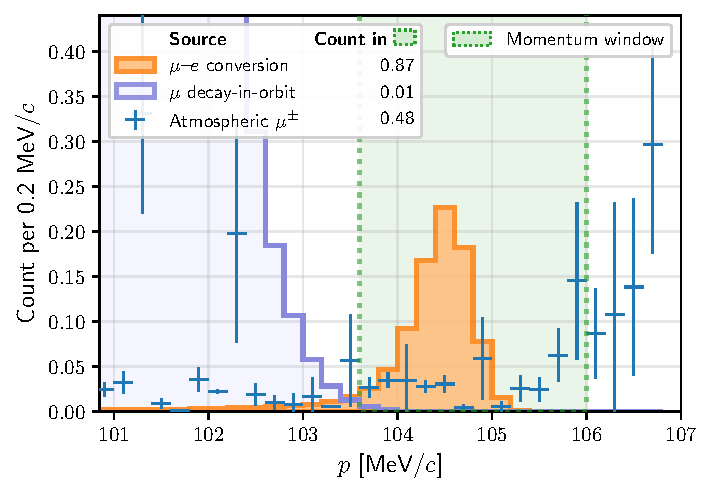
\includegraphics[width=\textwidth]{chapter6/thesis_conversion_search_momentum_distribution_withcuts_with_mu+_ID_dp=0.1_v3.pdf}
        \caption{With track direction identification: \SI{89}{\percent} of
        $\mu^+$-induced backgrounds are rejected and \SI{87}{\percent} of signal events
        are preserved.}
        \label{fig:spectrum_with_direction_id}
    \end{subfigure}
    \hfill
    \begin{subfigure}{0.48\textwidth}
        \centering
        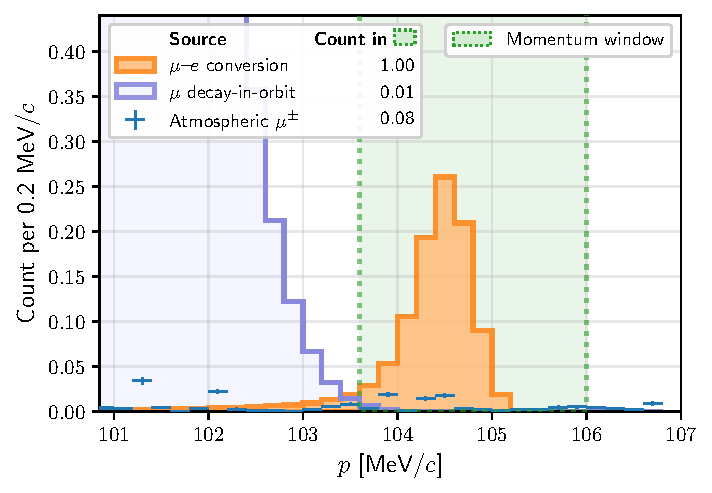
\includegraphics[width=\textwidth]{chapter6/thesis_conversion_search_momentum_distribution_withcuts_with_mu+-.pdf}
        \caption{With particle type identification by the Cherenkov layer of the
        CTH, assuming a $\mu^{\pm}$ rejection efficiency of \SI{99}{\percent}.}
        \label{fig:spectrum_with_cherenkov_pid}
    \end{subfigure}
        
    \caption{Signal and background event counts versus reconstructed track
    momentum, over $T_\mathrm{DAQ}=146$~days and assuming
    $\mathcal{B}_\mathrm{conversion} = 3.6\times 10^{-15}$. }
    \label{fig:lin_spectra}
\end{figure}


\subsection{CRV efficiency}

\begin{figure}
    \centering
    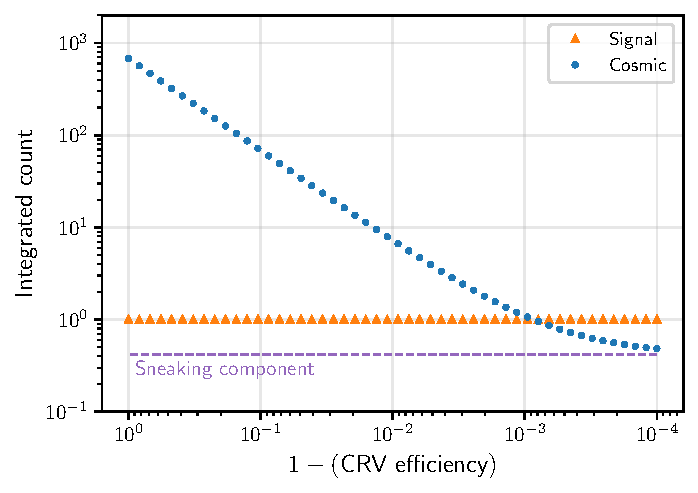
\includegraphics[width=0.5\textwidth]{chapter6/bg_count_vs_crv_efficiency.pdf}
    \caption[Integrated atmospheric background count versus CRV inefficiency]{ Integrated atmospheric background count versus CRV inefficiency
        (note the reversed horizontal axis), assuming no Cherenkov CTH layer and
        \SI{89}{\percent} $\mu^+$ rejection rate by direction identification.
        The lower bound arises from sneaking events, which are not detected by
        the CRV. 
        % More accurate particle identification by the CyDet helps to
        % reduce this sneaking component, e.g.\ by discriminating muons from
        % electrons.
        }
    \label{fig:bg_count_vs_crv_efficiency}
\end{figure}

The CRV efficiency determines the fraction of atmospheric events which can enter
the CyDet through the active parts of the CRV while not being vetoed. Although
we have assumed so far that the CRV successfully rejects \SI{99.99}{\percent} of
atmospheric muon events, this will not necessarily be realised in practice.
Figure~\ref{fig:bg_count_vs_crv_efficiency} shows the background event count as
a function of the CRV efficiency. An efficient CRV helps to reject the vast
majority of atmospheric backgrounds. An efficiency of at least
\SI{99.9}{\percent} seems necessary to suppress the background counts to fewer
than one. Beyond \SI{99.99}{\percent}, the contribution from sneaking events
becomes significant, and reducing the background rate is better tackled by means
of particle identification, such as with the Cherenkov CTH layer.

Table~\ref{tab:bg_summary} summarises the atmospheric background event counts
for $T_\mathrm{DAQ}=146$~days under various run conditions. Obviously, one major
aspect of identifying atmospheric muons is the CRV, and the background rate
greatly depends on its efficiency.

The problem caused by sneaking muons is more subtle. However, it can still
plague the conversion search by producing on the order of one signal-like event
during data acquisition. The most frequent sneaking backgrounds are produced by
anti-muons that disguise as negative particles by flying from the detector to the
muon stopping target. These events can, however, be distinguished from
conversion electrons via a direction identification technique using timing
information from the CDC and CTH. Being able to identify \SI{89}{\percent} of
$\mu^+$-induced events in this manner reduces the background counts to 1.10 with
a \SI{99.9}{\percent}-efficient CRV or 0.48 with a
\SI{99.99}{\percent}-efficient CRV. 

Eventually, when the CTH reaches its final stage with an outer Cherenkov layer,
muons will be more effectively distinguished from electrons. If the CTH allows us
to reject \SI{99}{\percent} of all $\mu^\pm$ events, the background count could
be as low as 0.08, with a \SI{99.99}{\percent}-efficient CRV.


\section{Discussion}


\begin{table}
    \centering\begin{tabular}{l|cc}
        \toprule
        \diagbox[width=4cm]{PID}{$\epsilon_\mathrm{CRV}$} & \SI{99.9}{\percent} & \SI{99.99}{\percent}\\\midrule
        None & 3.22 & 2.29 \\
        \SI{89}{\percent} $\mu^+$ (direction) & 1.10 & 0.48 \\
        \SI{99}{\percent} $\mu^\pm$ (Cherenkov) & 0.57 & {\bfseries 0.08} \\\bottomrule
    \end{tabular}
    \caption{ Summary of atmospheric background counts for
    $T_\mathrm{DAQ}=146$~days under different scenarios for particle
    identification (PID) and CRV efficiency ($\epsilon_\mathrm{CRV}$).}
    \label{tab:bg_summary}
\end{table}


\subsection{Summary}

In this chapter, we combined the BMC method with a $\mu$--$e$ conversion sample
and a DIO sample in order to determine how each process contributes in the event
counts recorded during the Phase\nobreakdash-I data acquisition run. The
analysis of signal events yields our estimate of the single event sensitivity of
the COMET Phase\nobreakdash-I experiment. Integrating over the entire run time
of Phase\nobreakdash-I, we find that atmospheric muon backgrounds outnumber the
next largest source of background, DIO, by an order of magnitude or more
depending on the exact conditions. The main factor in eliminating atmospheric
backgrounds is the efficiency of the CRV, followed by the CyDet system's ability
to distinguish between electrons and muons. In the absence of a
particle-identifying Cherenkov layer in the CTH, our results summarised in
Table~\ref{tab:bg_summary} suggest that the background count is at least 0.48
over 146 days, versus one signal event assuming $\mathcal{B}_\mathrm{conversion}
= 3.6 \times 10^{-15}$. With the final-stage CTH layout, the background count
falls to 0.08 assuming a \SI{99}{\percent} $\mu^\pm$ identification rate.

% Implications

% Use vs literature? Actually didn't do a lit review here in HEP...
Backward MC simulation is a powerful tool which enabled us to determine that
extremely rare conversion-like events can be produced by atmospheric muons
sneaking into the COMET detector system. These events can be an important
obstacle for the COMET Phase\nobreakdash-I conversion search if no additional way to
reject them, such as particle type identification, is put in place. Using a
standard MC simulation where events are generated far from the detector system,
those rare events that get past the CRV and produce signal-like tracks would
most likely not appear at all in the sample. Hence, the backward MC method is
absolutely key in this study and should continue to prove useful in COMET toward
Phase\nobreakdash-I and Phase\nobreakdash-II. More generally, any experiment searching for rare
processes and which is susceptible to cosmic ray-induced backgrounds will also
benefit from using backward MC to identify the kinds of atmospheric events that
are likely to mimic their signal, and estimate their frequency.

\subsection{Limitations and recommendations}


\subsubsection{Backward transport}
In our study, we used backward MC simulation to transport muons from the surface
of the CRV to the atmospheric plane. The assumption associated with this
procedure is that the muon is able to travel all the way from the atmospheric
source to the surface of the CRV. In reality, this assumption does not
necessarily hold and there is expected to be some fraction of atmospheric muons
which will interact close to the CRV and whose products will induce a background
event. These events do not contribute toward our results. Therefore, we are
underestimating the background rate from cosmic rays, but by how much is
difficult to determine. 

This bias could be addressed by sampling the muons not at the surface of the
CRV, but a little farther away. However, doing so would lead to more events
missing the detector, as is the case in forward MC, and therefore to wasted
computation. Already, in our study, very few sampled events pass the CyDet
selection criteria: around 1 in $10^5$ in the envelope sample, 1 in $10^7$ for
sneaking events. Pushing the sampling surface outward would decrease these
ratios and reduce our statistics further. Nevertheless, it can be done in the
future in order to estimate the extent of the bias.

\subsubsection{Sampling distributions}

Atmospheric muons are sampled around the CRV with arbitrary energy and direction
distributions. Our selection shows that only one event in \num{100000} produces
a fourfold coincidence and a track in the CyDet system. In a future iteration of
this study, one could determine if there is some region of the sampling phase
space which never contributes to the selected events: perhaps very high or very
low energy events, or events which are incident upon the CRV within a specific
range of azimuthal or zenith angle. Eliminating this region of phase space from
the sampling distribution function would increase the fraction of simulated
events which pass the selection, thus increasing the statistics on events of
interest for the same computational cost.


\subsubsection{Event selection}

To identify background candidates, events are selected that have a fourfold
coincidence in the CTH and an associated track in the CDC. When reconstructing a
trajectory, the track fitting algorithm ignores hits produced by other particles
in the CDC during the same event. Instead of using a track finding algorithm, we
use truth information from the MC simulation in order to select hits from the
right particle and provide them to the track fitting function. This has caused
at least one known inaccuracy in our study: events where a high energy muon
produces a shower in the CDC sometimes induce a fourfold coincidence, thus they
pass our selection criteria and may be counted as background events. In
realistic conditions, events that suddenly saturate a large fraction of CDC
channels, such as a high-energy shower, will most likely be discarded because
tracks cannot be reconstructed from the event. Therefore, these should not have
been counted as part of the integrated background, for instance in
Figures~\ref{fig:log_spectrum_nocuts} and~\ref{fig:bg_count_vs_crv_efficiency}.
These high energy muons typically fly straight through the CyDet system and hit
the CRV along the way. Hence, although this issue in our selection is likely to
have caused a slight overestimation of the total background rate, we expect the
sneaking component to be unaffected.

\subsubsection{Reconstruction and detector response}
Various aspects of our study are not faithful to the actual conditions of
Phase\nobreakdash-I. On the reconstruction side, for the atmospheric muon sample, we use a
helix fit to reconstruct the trajectory of each event where a fourfold
coincidence is produced. During data acquisition, a more complex fitting
algorithm, based on Kalman filtering, will be used. Similarly, for the
conversion and DIO samples, we do not perform reconstruction but naively
smear the true momentum of the track using the design momentum resolution of the
CDC. Because of those simplifications, we expect the resulting momentum spectra
to differ slightly in the real conditions of Phase\nobreakdash-I. 

Although ICEDUST has the capability to fully simulate each sub-detector's
response to incoming energy deposits, digitisation and calibration were not
simulated in this study. Instead, we simplified those processes by applying a
hardware efficiency factor to all samples. Similarly, the timing of events is
also disregarded in our simulation. Instead of assigning a realistic time of
production to conversion, DIO and atmospheric events, and then selecting events
that occur in the trigger time window, we apply an efficiency factor to each
sample based on their expected time distribution and the start and end time of
the trigger window. 

Hence, our study makes use of estimates based on other studies within the
collaboration, rather than conducting fully realistic calculations in the
detector response and reconstruction aspects. In future studies, and as
the Phase\nobreakdash-I data acquisition period approaches, it will be
especially important to rigorously simulate these effects to assess the
performance of the experiment as accurately as possible.
